\begin{tikzpicture}[%
  x=1.25cm,y=2cm,
  font=\footnotesize,
  imageNode/.style={inner sep=0pt},
  textAbove/.style={align=center, yshift=36mm},
  textBelow/.style={align=center, yshift=10.5mm}
  ]

\newcommand\fileImage[0]{
\includegraphics[width=.10\textwidth]{images/icon-file}}
\newcommand\metadataImage[0]{
\includegraphics[width=.12\textwidth]{images/metadata}}
\newcommand\astImage[0]{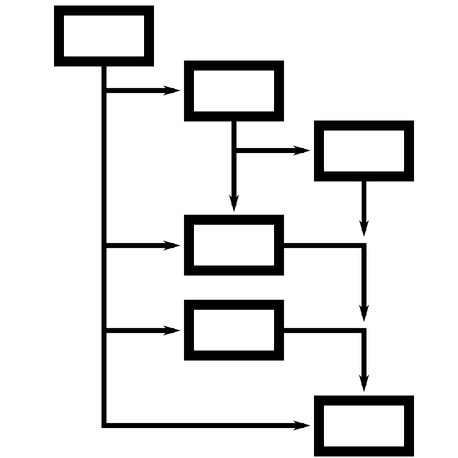
\includegraphics[width=.12\textwidth]{images/ast}}

\newcommand\drawFile[4][]{%
	\node[imageNode, #1] (#4) {\fileImage};
	\node[textAbove, below=of #4] {#2.#3};
}
\newcommand\ktFile[2][]{\drawFile[#1]{#2}{kt}{#2}}
\newcommand\jsFile[2][]{\drawFile[#1]{#2}{js}{#2}}
\newcommand\metaJsFile[2][]{\drawFile[#1]{#2}{meta.js}{meta#2}}

\newcommand\drawFileBelow[4][]{%
	\node[imageNode, #1] (#4) {\fileImage};
	\node[textBelow, below=of #4] {#2.#3};
}
\newcommand\ktFileBelow[2][]{\drawFileBelow[#1]{#2}{kt}{#2}}
\newcommand\jsFileBelow[2][]{\drawFileBelow[#1]{#2}{js}{#2}}
\newcommand\metaJsFileBelow[2][]{\drawFileBelow[#1]{#2}{meta.js}{meta#2}}

\newcommand\drawBoxWithOptions[4]{%
\begin{scope}[on background layer]
	\node[rounded corners, draw=black, very thick, dashed, fill=lightgray!10,
    	fit=#1,
    	label={[yshift=0mm]#2},
    	#4
    ] (#3) {};
\end{scope}
}

\newcommand\drawBox[3]{\drawBoxWithOptions{#1}{#2}{#3}{inner ysep=5mm, inner xsep=3mm}}

\ktFile{main}
\ktFile[right=of main, xshift=-5mm]{util}
\drawBox{(main)(util)}{Программа}{ktFiles}

\metaJsFile[right=of ktFiles, xshift=5mm]{lib}
\jsFile[right=of metalib, xshift=-5mm]{lib}
\drawBox{(lib)(metalib)}{Библиотека}{jsFiles}

\node[imageNode, below=of metalib, yshift=-15mm] (libraryMetadata) {\metadataImage};
\node[xshift=10mm, left=of libraryMetadata,align=center] {Метаданные\\библиотеки};

\node[imageNode, below=of ktFiles, yshift=-10mm] (ktAst) {\astImage};
\node[xshift=10mm, left=of ktAst] (ktAstText) {Kotlin AST};

\node[imageNode, below=of ktAst,yshift=-10mm] (programMetadata) {\metadataImage};
\node[xshift=10mm, left=of programMetadata,align=center] (programMetadataText) {Метаданные\\программы};

\drawBox{(programMetadata)(programMetadataText)(ktAstText)(libraryMetadata)}{}{codegenInput}

\node[imageNode, right=of codegenInput, xshift=21mm, yshift=20mm] (jsAst) {\astImage};
\node[above=of jsAst, yshift=-8mm] (jsAstText) {JavaScript AST};

\metaJsFileBelow[right=of programMetadata,xshift=50mm]{program}
\jsFileBelow[right=of metaprogram, xshift=-5mm]{program}
\drawBoxWithOptions{(program)(metaprogram)}{}{output}{inner sep=5mm}

% Arrows
\tikzstyle{fatArrow}=[line width=1mm,-triangle 90,postaction={draw, line width=3mm, shorten >=1.4mm, -}]
\draw [fatArrow](ktFiles.south) -- node[anchor=west,align=center, yshift=2mm] {~(1) Синтаксический\\анализ} (ktAst.north);
\draw [fatArrow](metalib.south) -- node[anchor=west,align=center, yshift=1mm] {~(2) Десериализация} (libraryMetadata.north);
\draw [fatArrow](ktAst.south) -- node[anchor=west,align=center] {~(3) Семантический\\анализ} (programMetadata.north);
\draw [fatArrow]($(codegenInput.east) + (0,1)$) -- node[anchor=north,align=center,yshift=-2mm,xshift=0mm] {(4) Трансляция} (jsAst.west);
\draw [fatArrow](jsAst.south) -- node[anchor=west,align=center,yshift=3mm] {~(5) Сериализция} (program.north);
\draw [fatArrow](programMetadata.east) -- node[anchor=north,align=center,yshift=-2mm,xshift=-10mm] {~(6) Сериализция} (metaprogram.west);

\end{tikzpicture}
